%; whizzy chapter
% -initex iniptex -latex platex -format platex -bibtex jbibtex -fmt fmt
% 以上 whizzytex を使用する場合の設定。

%     Kansai Debian Meeting resources
%     Copyright (C) 2007 Takaya Yamashita
%     Thank you for Tokyo Debian Meeting resources

%     This program is free software; you can redistribute it and/or modify
%     it under the terms of the GNU General Public License as published by
%     the Free Software Foundation; either version 2 of the License, or
%     (at your option) any later version.

%     This program is distributed in the hope that it will be useful,
%     but WITHOUT ANY WARRANTY; without even the implied warranty of
%     MERCHANTABILITY or FITNESS FOR A PARTICULAR PURPOSE.  See the
%     GNU General Public License for more details.

%     You should have received a copy of the GNU General Public License
%     along with this program; if not, write to the Free Software
%     Foundation, Inc., 51 Franklin St, Fifth Floor, Boston, MA  02110-1301 USA

%  preview (shell-command (concat "evince " (replace-regexp-in-string "tex$" "pdf"(buffer-file-name)) "&"))
% 画像ファイルを処理するためにはebbを利用してboundingboxを作成。
%(shell-command "cd image200708; ebb *.png")

%%ここからヘッダ開始。

\documentclass[mingoth,a4paper]{jsarticle}
\usepackage{kansaimonthlyreport}
\usepackage{ascmac}

% 日付を定義する、毎月変わります。
\newcommand{\debmtgyear}{2008}
\newcommand{\debmtgdate}{27}
\newcommand{\debmtgmonth}{9}
\newcommand{\debmtgnumber}{17}

\begin{document}

\begin{titlepage}

% 毎月変更する部分、本文の末尾も修正することをわすれずに

 第\debmtgnumber{}回 関西 Debian 勉強会資料

\vspace{2cm}

\begin{center}
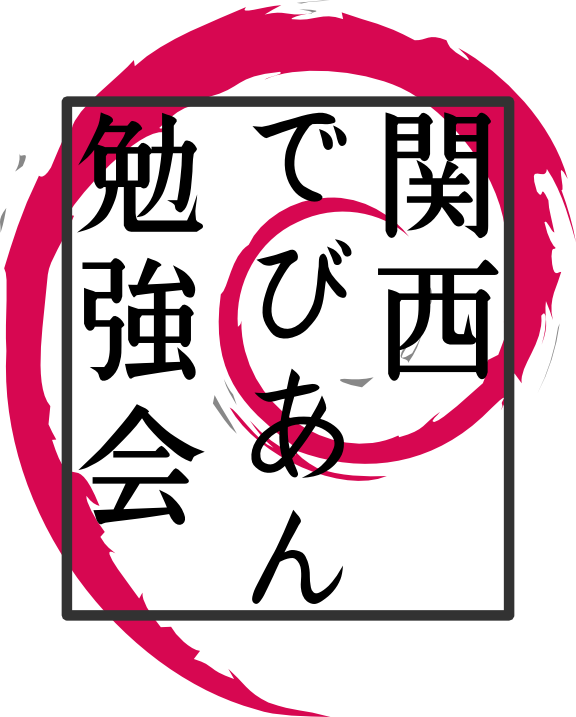
\includegraphics{image200802/kansaidebianlogo.png}
\end{center}

\begin{flushright}
\hfill{}関西 Debian 勉強会担当者 山下 尊也\\
\hfill{}\debmtgyear{}年\debmtgmonth{}月\debmtgdate{}日
\end{flushright}

\thispagestyle{empty}
\end{titlepage}

\dancersection{Introduction}{山下 尊也}
 
 関西 Debian 勉強会はDebian GNU/Linux のさまざ
 まなトピック(新しいパッケージ、Debian 特有の機能の仕組、Debian 界隈で起
 こった出来事、などなど)について話し合う会です。

 目的として次の三つを考えています。
 \begin{itemize}
  \item MLや掲示板ではなく、直接顔を合わせる事での情報交換の促進
  \item 定期的に集まれる場所
  \item 資料の作成
 \end{itemize}

 それでは、楽しい一時をお楽しみ下さい。

\newpage

\begin{minipage}[b]{0.2\hsize}
 {\rotatebox{90}{\fontsize{80}{80}
{\gt 関西デビアン勉強会}}}
\end{minipage}
\begin{minipage}[b]{0.8\hsize}
\hrule
\vspace{2mm}
\hrule
\setcounter{tocdepth}{1}
\tableofcontents
\vspace{2mm}
\hrule
\end{minipage}

\dancersection{最近のDebian関係のイベント報告}{山下 尊也}

\subsection{第16回 関西 Debian 勉強会}

2008年8月17日に「第16回 関西 Debian 勉強会」を行いました。

「Debian を Windows な PC でも楽しもう 〜応用編〜」と言うことで、
4月にあった、基礎編の延長線上にある応用編を名村さんにやって頂きました。
名村さんは、お子さんが産まれたようで、
嬉しそうにお子さんの写真を見せながら、講師をして頂きました。

そして、私から、「オープンソースカンファレンス2008 Kansai を振り返る」
と言うことで、反省点などを話させて頂きました。

また、臨時講師として、久保さんから「DNS のキャッシュ汚染問題について」
を話をして頂き、最後に、\url{http://wiki.debian.org/NewInLenny} を見て、
討論を行いました。
大勢の方と見る事で、
一人では気づかなかった新しい点なども気づいたと思います。

16人来る予定でしたが、無断欠席が3人いました。
資料を印刷する際の費用なども考えて頂き、必ず欠席の際は、
私にメールをして欲しいです。

%% takaya
\dancersection{Debian Live に Ubiquity を移植できるか?}{山下 尊也}
\label{sec:ubiquity}

% \subsection{Ubiquityって何してるの?}

% Ubiquity is a simple graphical live CD installer designed to integrate
% well with Debian- and Ubuntu-based systems、 written largely in Python、
% using d-i as a backend for many of its functions for ease of
% maintenance。

% Ubiquityは大部分がPythonで書かれており、
% メンテナンスの簡潔さのためにそのほとんどの関数を Debian Installer を使用
% しております。Debian と Ubuntu ベースのシステムでLive CDに統合したデザイ
% ンのインストーラです。

\subsection{Ubiquityパッケージをビルドする}

\url{http://jp.archive.ubuntu.com/ubuntu/}からubiquityのソースを取って
きます。

今回、私は、
{\tt ubiquity\_1.8.12.tar.gz}
をダウンロードしてきました。

なんとか、snapshot.debianやソースパッケージを用いて、依存関係を解決しま
した。\footnote{rulesの変更だけしたら大丈夫かも?本来はちゃんとした依存
関係を調べないといけません。}

しかし、ビルドの行程で、
{\tt /usr/share/iso-codes/iso\_3166.tab}
が存在しないと怒られます。
{\tt iso\_3166.tab}
は、地理情報を表しているものです。
調べてみたところ、sargeやetchにはiso-3166-udebと言う形で提供されています
が、lennyからは、iso-3166-udebパッケージが廃止されています。

調べていく過程で、tzdataパッケージに、
iso3166.tabと言うファイルが存在する事が分かりました。
中身を見たところ、これを利用すればDebianでもビルド出来そうです。
今回は、時間がなかったため、
{\tt iso\_3166.tab}
をUbuntu Hardyが起動している環境から持ってきて、利用しました。

なんとか、以下のパッケージを作成する事が出来ました。
\begin{itemize}
 \item {\tt ubiquity-frontend-gtk\_1.8.12\_i386.deb}
 \item {\tt ubiquity-frontend-kde\_1.8.12\_all.deb}
 \item {\tt ubiquity-frontend-mythbuntu\_1.8.12\_all.deb}
 \item {\tt ubiquity-ubuntu-artwork\_1.8.12\_all.deb}
 \item {\tt ubiquity\_1.8.12\_i386.deb}
\end{itemize}

また、
{\tt d-i/source/localechooser/mkshort}
を変更し、
{\tt /usr/share/zoneinfo/iso3166.tab}
を用いる変更を加えれば、
この問題は解決出来そうです。

\subsection{Ubiquity で必要になるパッケージ}

\subsubsection{Ubiquity 関係パッケージの Depends で関係するもの}
\label{sec:depends}

Ubuntu Hardyが起動している環境から、
{\tt /var/lib/apt/lists/}
ディレクトリ下にある

{\tt jp.archive.ubuntu.com\_ubuntu\_dists\_hardy\_main\_binary-i386\_Packages}

を持ってきて、ubiquity関連パッケージのDependsに書かれている
ものを書き出したものが以下のものです。

\begin{commandline}
adduser
console-setup
debconf
grub
iso-codes
kwin
laptop-detect
libatk1.0-0
libc6
libcairo2
libdebconfclient0
libdebian-installer4
libffi4
libglib2.0-0
libgtk2.0-0
libpango1.0-0
libparted1.7-1
libxml2
lsb-release
os-prober
passwd
python
python-apt
python-central
python-glade2
python-gtk2
python-qt4
sudo
ubiquity
ubiquity-artwork-1.8.7
ubiquity-casper
ubiquity-frontend-1.8.7
x-window-manager
\end{commandline}

同様に、Debian Lennyが動いている環境の{\tt /var/lib/apt/lists/}にある

\begin{itemize}
 \item {\tt cdn.debian.or.jp\_debian\_dists\_lenny\_main\_binary-i386\_Packages}
 \item {\tt cdn.debian.or.jp\_debian\_dists\_lenny\_contrib\_binary-i386\_Packages}
 \item {\tt cdn.debian.or.jp\_debian\_dists\_lenny\_non-free\_binary-i386\_Packages}
\end{itemize}

をチェックしたところ、Debian Lennyには以下のパッケージが存在しない事が
分かりました。

\begin{commandline}
libffi4
libparted1.7-1
ubiquity
ubiquity-artwork-1.8.7
ubiquity-casper
ubiquity-frontend-1.8.7
x-window-manager
\end{commandline}

libffi4は、etchに存在し、
libparted1.7-1は、ソースからビルドすれば、パッケージの作成をする事が出来
ます。\footnote{現在、automake1.8とのバグのため、ビルド出来ない状況になっ
ているため、今回は、snapshot.debianからパッケージをダウンロードしました。}

x-window-managerは仮想パッケージのため、このリストには存在しません。
と言うことで、依存関係は解決出来たみたいです。

\subsection{Debian Liveに依存関係を解決し、入れてみる}

OSC Kansaiで配布したDebian Liveで使われていたものをある程度、
利用したいため、git hubから取ってきて、\ref{sec:depends}で追加したリストを追記します。

\begin{commandline}
 % git clone git://github.com/nogajun/debian-study-live-cd.git
 % vi debian-study-live-cd/config/chroot_local-packageslists/06-ubiquity
\end{commandline}

また、GTKの環境だけを考えているため、以下のパッケージをインストールする事を考
えます。

\begin{commandline}
ubiquity-frontend-gtk_1.8.12_i386.deb
ubiquity-ubuntu-artwork_1.8.12_all.deb
ubiquity_1.8.12_i386.deb 
\end{commandline}

% \verb|debian-study-live-cd/config/chroot_local-packages|
{\tt debian-study-live-cd/config/chroot\_local-packages|}
ディレクトリに入れ、パッケージの正当性チェックを無効にしておきます。

\begin{commandline}
 % sudo lh_build
\end{commandline}

しかし、ここでまたもや、依存関係のエラーがでます。

\begin{commandline}
  libffi4: Depends: gcc-4.1-base (= 4.1.1-21) but it is not going to be installed
  ubiquity: Depends: ubiquity-casper but it is not installable 
\end{commandline}

とりあえず、リストの前に追加しますが、ubiquity-casperは、Ubuntuにしかあ
りません。
ubiquity-casperは、live installerからの設定を行うものですが、
これをソースからビルドすると

\begin{commandline}
Some packages could not be installed. This may mean that you have
requested an impossible situation or if you are using the unstable
distribution that some required packages have not yet been created
or been moved out of Incoming.
The following information may help to resolve the situation:
 casper: Depends: busybox-initramfs (>= 1:1.1.3-4ubuntu3) but it is not installable
         Depends: localechooser-data but it is not installable
 libffi4: Depends: gcc-4.1-base (= 4.1.1-21) but it is not going to be installed
E: Broken packages
\end{commandline}

Ubiquityの問題ではなく、依存関係をどうするかを考えた方が良かったみたいで
す。少しずつ時間を見つけて、依存関係を見直していこうと思います。

\dancersection{10分でわかる Debianフリーソフトウェアガイドライン (DFSG)}{木下 達也}
\subsection{Debianフリーソフトウェアガイドラインとは}

ある著作物が「フリー」かどうか、
フリー(自由な)OSであるDebianの構成要素として
適しているかどうかを判定する際の基準、それが
Debianフリーソフトウェアガイドライン
(DFSG: Debian Free Software Guidelines)です。

\url{http://www.debian.org/social_contract#guidelines}
 
フリー(自由な)ソフトウェアとは、自由に使ったり、
変更したり、コピーして配ったりできるソフトウェアの
ことをいいます。

ただし、「自由」とはいっても、無制限というわけではなく、
ある種の制約は認められています。
(著作権表示・ライセンスの維持、変更の明示など)

\subsection{著作権とライセンス}

著作物には、基本的に著作者に対して「著作権」
が発生しています。

つまり、著作物を変更したりコピーして配ったりするには、
著作者からの許可(ライセンス)が必要になります。

ライセンスは次のように確認します。

\begin{itemize}
 \item 変更や配布が許可されているか
 \item それらに付随する制約はどうか
\end{itemize}

その他、個別の事情も検討する必要があります。
(特許、商標など)

\newpage
\subsection{Debianフリーソフトウェアガイドラインの説明}

\begin{itemize}
 \item 1. 自由な再配布 (Free Redistribution)

有償・無償を問わず、
別途の許可を必要とすることなく、
プログラムを複数まとめて配布できる。

(Artistic License: プログラム単体への課金は禁止、複数まとめての販売は可)

 \item 2. ソースコード (Source Code)

ソースコード(変更に適した形式)が必要。

実行形式だけでなくソースコードでも配布できる。

 \item 3. 派生ソフトウェア (Derived Works)

同様のライセンスで変更版を配布できる。

(GNU GPL: 変更版全体に同様のライセンスを強制)

(BSD License: 変更版全体には別ライセンスの適用可)

 \item 4. 原作者によるソースコードの整合性維持
   (Integrity of The Author's Source Code)

変更版のソースコードを配布する場合に、
元のソースコードと差分(パッチ)という形式のみ許可
という制約は許容、ただし非推奨。

(QPL: 元のソースコードと差分の要求)

 \item 5. すべての個人、団体の平等
   (No Discrimination Against Persons or Groups)

いかなる個人・団体も差別せずに許可。

 \item 6. 目標分野の平等
   (No Discrimination Against Fields of Endeavor)

商用・非商用・平和利用・軍事目的など、用途を制限しない。

 \item 7. ライセンスの配布
   (Distribution of License)

ライセンスは、再配布されたすべての人々に、
別途の許可を必要とすることなく、適用される。

 \item 8. ライセンスはDebianに限定されない
   (License Must Not Be Specific to Debian)

Debianの一部としてのみの許可ではなく、
他のシステムにも適用できるように。
特定の製品に依存しないように。

 \item 9. ライセンスは他のソフトウエアを侵害しない
   (License Must Not Contaminate Other Software)

たとえば、同じ媒体で配布されるソフトウエアすべてが
フリーソフトウエアであることを要求しないように。

 \item 10. フリーなライセンスの例
   (Example Licenses)

GNU GPL, BSD License, Artistic License

(私見としては、Artistic Licenseは推奨しません。
Free Software Foundationでは「曖昧過ぎる」としてNon-Freeに分類されています)

\url{http://www.gnu.org/licenses/license-list.ja.html#ArtisticLicense}

\end{itemize}

\dancersection{今後の予定}{山下 尊也}

\subsection{次回}
次回は、2008年11月7日,8日に行われる
関西オープンフォーラム\footnote{\url{http://k-of.jp/}}にて開催する予定です。

\subsection{KDRのおしらせ}
関西Debian勉強会の有志で
関西Debian勉強会とは独立した形で、
週に一度、読書会(KDR)を開いています。
詳しくはKDR公開用ページ\footnote{\url{http://qwik.jp/kdrweb/}}
をご覧下さい。

\dancersection{メモ}{}
\mbox{}\newpage

\printindex
 \cleartooddpage

 \begin{minipage}[b]{0.2\hsize}
  \rotatebox{90}{\fontsize{80}{80} {\gt 関西デビアン勉強会} }
 \end{minipage}
 \begin{minipage}[b]{0.8\hsize}

 \vspace*{15cm}
 \rule{\hsize}{1mm}
 \vspace{2mm}
 
\includegraphics[width=2cm]{image200502/openlogo-nd.eps}
 \noindent \Large \bf Debian 勉強会資料\\ \\
 \noindent \normalfont \debmtgyear{}年\debmtgmonth{}月\debmtgdate{}日 \hspace{5mm}  初版第1刷発行\\
 \noindent \normalfont 関西 Debian 勉強会 (編集・印刷・発行)\\
 \rule{\hsize}{1mm}
 \end{minipage}

\end{document}
